\chapter{METHODOLOGY}
This chapter is composed of four sections.
Section \ref{meth:som} describes PySOM, our own graph based implementation of
SOM. PySOM provides the necessary inputs to our three diagnostics as described
in section \ref{meth:diag}.  These diagnostics were developed to help
understand how irregularities in topology effect the SOM. To use these
diagnostics we must train several SOMs with comparable training data and
parameters.  The specifics of our training data are explained in section
\ref{meth:data}.  Section \ref{meth:train} describes the training parameters used
across all of our SOMs.

\section{Graph Based Implementation of SOM}
\label{meth:som}
The most widely available implementation of SOM is Kohonen's
own SOM\_PAK \citep{kohonen1996}.  SOM\_PAK implements both the traditional
rectangular and hexagonal topologies.  However, implementations of the
geodesic and spherical SOMs were not readily available at the time this thesis
was written.  In order to test these topologies it was necessary to implement
our own version of SOM, PySOM.  Because the goal of this thesis was to study
different topologies for use in SOM, we created PySOM to be independent from
the topology.
That is, our implementation is not explicitly aware of the topology.  Rather, we
represent the topology of the SOM as a graph. The graph provides the necessary
information to determine neuron adjacency and construct neighborhoods.  The
nodes in the graph are pointers to the reference vectors ($m_i$).

To allow for rapid development and cross-platform support we choose to write PySOM
in the Python programing language. As noted by \cite{Rey2006} Python is an
object-oriented programing language that is becoming increasingly popular in
scientific computing. PySOM is maintained as an open-source project in hopes
of facilitating collaboration and further research.  In its present form,
PySOM has no user interface, however it is written as a Python library which
allows all of its functionality to be accessed programmatically. %spell checked with google
Python also provides an interactive interpreter which may be used to access
PySOM in a command line environment.

By abstracting the topology, PySOM can train a SOM using any topology for
which a graph structure can be created. We leverage an existing graph library,
NetworkX, to represent our topologies \citep{networkx}.  Our neighborhood
functions are built on top of this library.  Apart from our neighborhood
search functions, our implementation follows the original incremental SOM
algorithm that is described by \cite{Kohonen2000}.  We store our trained SOM
in a similar fashion as SOM\_PAK.  The reference vectors are represented in a
simple text file.  These ``codebook'' files contain a description of the
topology and other training parameters in the first line of the file.  Each
subsequent line lists the values for the parametric reference vectors, $m_i$,
of the SOM's neurons \citep{kohonen1996}. In addition to this codebook file we
also store the graph as a serialized Python object.  Creating the graph
structures for the spherical topologies is considerably more complex and
requires more computation than the traditional topologies.

We provide utility functions to create the graph structures for both the
rectangular and hexagonal topologies.  As shown in figure \ref{flowchart}, to create the graph structure for the
geodesic topology we use the ``dome'' software package, which creates a
``WRL'' file containing the points coordinates for each node in the geodesic
dome \citep{dome}.  These coordinates are fed into the STRIPACK software
program.  STRIPACK computes both the Voronoi cells and their complement, the
Delaunay triangulation, on the surface of the sphere \citep{Ranka97}.  We
provide a utility script, which converts the WRL file format into
the XYZ file format that STRIPACK expects.  The Delaunay triangulation provides the graph
structure between the neurons of the geodesic SOM.  A similar process is used
for the spherical topology. In this case we wrote a Python implementation of
the method for distributing points on a sphere that was introduced by
\cite{Rakhmanov94}.  Once again the coordinates are fed into STRIPACK.
An additional utility program reads the output from STRIPACK and
creates the NetworkX graph structure.  PySOM has no direct graphical
output, however several utility functions are provided to assist in the
creation of visualizations.  These functions create text files that are compatible with
popular GIS software packages, namely ESRI's ArcGIS.  ArcGIS provides tools to
create ShapeFiles from these text files.

\begin{figure}[htb]
\centering
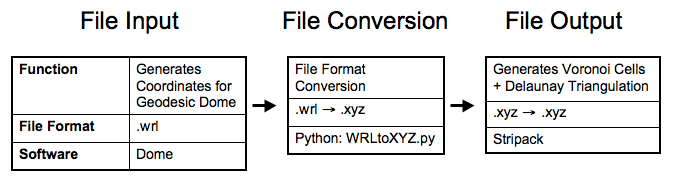
\includegraphics[width=.9\linewidth]{flowchart.png}
\caption{Steps for creating geodesic graph structures.}
\label{flowchart}
\end{figure}

\section{Diagnostics}
\label{meth:diag}
In traditional SOMs, outlying observations are pushed to the edge of the map
where they encounter fewer competing signals.  A prime example of this is the
``Utah-Hawaii'' case shown in Figure \ref{som:states}.  Relying only on the
SOM, one would be left to believe that the two states are similar.  Recalling
that the QError measures the distance between two vectors in attribute space,
we calculate that the QError from Utah to the neuron is $1.509$, the QError from
Hawaii to the neuron in $1.505$, but the QError from Utah to Hawaii is
$3.014$. In this case only Utah and Hawaii were mapped to that neuron.  In a
case where multiple observations land on the same neuron, it is possible to
measure the average pairwise QErrors between those observations.  This gives us a
notion of internal heterogeneity, \(H\), for each neuron.  We define the
internal heterogeneity of neuron \(i\) as,
 \begin{equation}
   {H_i} = \frac{2}{{n_i}^2-{n_i}}\sum_{j=1}^{n_i}\sum_{k=j+1}^{n_i} ||{x_{ij}}-{x_{ik}}||
 \label{eqno1}
 \end{equation}
where, \(n_i\) is the number of observations mapped to \(i\), and \(x_i\) are
the input vectors mapped to \(i\).   The double bars represent the Euclidean
distance between two observations which are references by \(j\) and \(k\). We
divide the sum of these distances by the number of pair-wise comparisons.
For any neuron that captures more then one observation, this measure tells how
dissimilar those observations are. 

The edge effects in SOM make it clear that the compression of the input-space is
not uniform throughout a trained map.  While outliers being pushed to the edge of
the SOM is not necessarily an undesirable outcome, it is important to understand
when and where information is being compressed.  This variable compression of
the input-space is what allows the SOM to represent high-dimensional data, but
it can also mislead the viewer.  Observing the internal heterogeneity of
neurons may shed light on the patterns of compression.  

More specifically we have developed diagnostics that explore how irregularities
in the topology of the SOM effect this internal heterogeneity.  We compare the
internal heterogeneity at the scale of the neuron and the overall map.  Each
diagnostic was designed to answer a specific research question.  The first
diagnostic addresses the research question regarding the internal
heterogeneity and neighborhood size.  The second diagnostic addresses the
question concerning internal heterogeneity and topological irregularity.  The
third helps visualize the patterns between internal heterogeneity; the
usefulness of which is examined in the next chapter.

\subsection{Internal Heterogeneity vs. First-Order Neighborhood Size}
\label{q1}
This diagnostic compares the internal heterogeneity of each neuron against
the neuron's first-order neighborhood size.  It would be expected that in
traditional SOMs neurons closer to the edge, those with fewer neighbors, will
have higher internal heterogeneity. Neurons on the edge of the traditional
(rectangular and hexagonal) topologies are considered more irregular, because
they have fewer neighbors than neurons inside the edge.  This can be extended to
spherical SOMs by considering the degree of any given neuron.  The degree of a
neuron $deg(m_i)$ measures the number of adjacent neurons.  If the
relationship between $H_i$ and $deg(m_i)$ is consistent across topologies,
we would expect neurons with lower degrees to display higher internal heterogeneity.

To implement this diagnostic we calculate the internal heterogeneity ($H_i$)
and degree ($deg(m_i)$) of each neuron. The neurons are then separated into a small number of
groups based on the degree.  For most topologies the number of
different degrees will be limited to three or four.  The variance and mean
is calculated for each of these groups.  The expected result is that
variances and means of the groups will decrease as the degree increases.  This
hypothesis is tested using random labeling as described by \cite{siss2004}.
In random labeling, we randomly assign our calculated $H$ values to the
neurons and recompute the mean and variance of the groups.  We do this many times,
9999 in our case, in order to approximate the distribution under the null
hypothesis that there is no relationship between the degree of a neuron and
its internal heterogeneity. Finally we
calculate pseudo p-values by comparing our observed mean and variance values
with the simulated distributions.  The results are also visualized using
box-and-whisker diagrams. Box-and-whisker diagrams, or box plots, show the
properties of a distribution.  The diagram shows the mean, first and second
standard deviations, and outliers that extend beyond the second deviation.

One problem that we face in this diagnostic is a small sample size when the neurons of a given
SOM are grouped by their degree.  For example, the four corners of the
rectangular topology are the only neurons that have a degree of two.  The rest
of the neurons have three or four neighbors depending on whether or not they
are on the edge. To address the problem of small sample size for topologies
with relatively few neurons of a particular degree, we will increase
the sample size by combining the results of many SOMs.

\subsection{Internal Heterogeneity vs. Topological Regularity}
This diagnostic compares the internal heterogeneity of each neuron against a
measure of regularity for its associated topology.  As mentioned above the
degree of each neuron measures the number of adjacent neighbors.  A completely
regular network topology (i.e. the torus) has no variance between these
measures.  For irregular networks the variance between these degrees gives us
a measure of irregularity. This particular measure is known as degree
centrality.  The degree of a node on a network is a measure of its centrality, or
importance. Nodes with more connections are thought to be more central to the
network and have a larger influence than nodes with fewer connections.

This holds with our understanding of the edge effect.  Neurons on the edge are
less central to the network and have less influence on training than other nodes.  These
edge nodes are also less influenced by the network, allowing outliers take
root.  During the training process, observations that are more average than
others tend to be centralized.  More extreme observations tend to be pushed to
the edges.  Referring back to figure \ref{som:states}, you'll notice
that observations with smaller symbols are closer to the mean of the
input-space and that these observations have been centralized in the network.
Using the degree as a measure of centrality does not capture this picture
well, as neurons near the edge can still have a large degree.  A better way to
capture this effect is to look at closeness centrality, which is the
inverse of the average distance of a neuron to every other neuron on the
network \citep{Wasserman:1994}.

Closeness centrality provides a more complete measure of connectedness in a
given topology than degree centrality.  In this diagnostic we compare the
internal heterogeneity of the neurons against the average closeness centrality
of their respective topologies.  This results in one group of internal
heterogeneity measurements for each topology tested.  We evaluated this
diagnostic in much the same way as the last.  We compare the variances and
means of each group, testing for differences with random labeling.  It is
expected that the distribution of internal heterogeneity will be narrower for
groups trained on more regular topologies.  It is further hypothesized that
the mean of internal heterogeneity will decrease when the network is more
regular.  %In addition to testing these assumptions with random labeling we
%visualize the results with box plots.

\subsection{Visualize Internal Heterogeneity Mapping}
Visualizing the internal heterogeneity may yield insight into how irregular topology
effects the SOM.  Creating these visualization for many different topologies
however, offers a number of challenges.  While the rectangular and hexagonal
topologies are rather straight forward to visualize, the spherical and geodesic
topologies are significantly more involved.  In order to leverage the utility
of existing GIS software we represent our topologies in a form that
these software packages understand.  Toward that end we create polygon layers
in which each polygon represents a neuron.  Shared borders represent
connections between neurons.  Creating the polygons for these topologies
required that we first compute the Voronoi diagram on the surface of the
sphere.  This is done using STRIPACK, a software program created by
\cite{Ranka97}.  Despite the prevalence of spherical coordinates
in GIS, modern GIS software packages have their roots in CAD software. As such
they all assume Cartesian distances and thus can not handle polygons that
cross the $180^{th}$ meridian.  To accommodate this we split each polygon at
the $180^{th}$ meridian and redraw it as two parts.

Once the GIS layers have been created and the internal heterogeneity of each
neuron has been calculated, a number of visualizations become possible. We
visualize the internal heterogeneity by shading the corresponding polygons.
These visualizations allow for the exploration of patterns in internal
heterogeneity with relation to the underlaying topology.  Further, we can
visualize the component planes, which show how the higher dimensions are
represented in the various SOMs.  We also map our synthetic data back onto the SOM in
order to calculate cluster membership of the neurons.  Visualizing cluster
membership clearly shows how the various topologies perform clustering.


\section{Data}
\label{meth:data}
%Comment from Skupin...
%This section is obviously leaving most of the specifics of the synthetic data
%generation out, which is problematic. I'm willing to go along with this for
%the proposal though, unless it gets raised by the third committee member
Our internal heterogeneity measure is sensitive to both the properties of the SOM
and the properties of the training data. Therefore, a dataset with uniform
properties is needed. We follow the method for generating uniform synthetic
data used by \cite{wu2006}.  Their method creates seven clusters in three
dimensions.  The uniform clusters generated by this method allow us to
systematically compare the diagnostics under several different topologies.
Each cluster is normally distributed and has a standard deviation of one.  The
clusters are centered at the origin and ten units out in each directions on
the x, y and z axes. To ensure that we can calculate an internal heterogeneity
for as many neurons as possible, we create approximately $25,000$ observations
in each dataset.  As described in the next section, our SOMs have either 642
or 644 neurons (depending on the topology).  Having a large number of
observation relative to the number of neurons will force the SOM to perform
clustering, increasing the number of neurons for which the internal
heterogeneity can be computed.

As mentioned in section \ref{q1} we will need to combine the results of
multiple SOMs in order to ensure a large enough sample size.  To accomplish
this we will create ten synthetic datasets as described above.  Each of these
datasets can be thought of as samples from the same input space.  That is, the
data generating process remains the same for each synthetic dataset created.
After training ten SOMs for each topology we take the average internal
heterogeneity of each trained SOM.  We compare these results to ensure that
trained SOMs behave similarly within each topology.


%We will create a number of different data sets and use them to train various SOMs.  

%the data is generated in such a way to increase the probability that each neuron will be occupied by more than one observation.

%Initially the synthetic data for this thesis came from a Gaussian cluster
%generator which creates clusters by randomly sampling from multivariate
%normal distributions \citep{handl}.  \citeauthor{handl}' method to keep
%clusters from overlapping is to create one cluster at a time, with each new
%cluster checked to see if it overlaps with an existing cluster. If it does,
%it is rejected.  The generator continues until the desired number of
%non-overlapping clusters has been reached.  This method tends to create
%clusters of very different shapes and sizes (or extents).

%The limit to using this method for creating data became evident when we
%realized that the internal variance measure was being affected by the
%structure of the clusters.  The internal variance essentially looks at the
%portion of a cluster that is mapped to a particular neuron and measures the
%density.  Because we specify that each cluster contain an equal number of
%observations, they tend to get equal representation (in terms of number of
%neurons) on the trained SOM.  The result of all this is that the smaller,
%more dense clusters display very low internal variance relative to the
%larger, less dense clusters.  While this may have interesting consequences in
%other applications, because of these effects on the internal variance our
%ability to determine how changes in the topology are affecting the meassure.
%because it interferes with the measurement of internal variance, we had to
%adopt another method of synthetic data generation. 



\section{Training Parameters}
\label{meth:train}
Before we can go on to address the research questions we need to train a
series of SOMs.  We train SOMs using four different topologies:
\emph{rectangular, hexagonal, geodesic sphere} and \emph{spherical}.  The spherical
topology is based on a method, developed by \cite{Rakhmanov94}, for
distributing an arbitrary number of points on to the surface of a sphere.
Delaunay triangulation is then applied to these points, producing a
topological structure.  To yield meaningful results these SOMs must be trained
with comparable parameters.  The literature provides many rules of thumb for
training a SOM: each SOM is trained in two stages, the first of which uses a larger
initial learning rate and neighborhood search radius with a small number of
training steps; the second stage uses a lower initial learning rate and
neighborhood search radius, but extends the length of training. In PySOM we
define the initial neighborhood search radius as a percentage of the maximum
width of the graph.
\\
First Stage Parameters:
\begin{itemize}
  \item Initial neighborhood search radius of 50\%, which decreases during training. 
  \item Initial learning rate of 0.04 which decreases during training.
  \item 100,000 training steps.
\end{itemize}
Second Stage Parameters:
\begin{itemize}
  \item Initial neighborhood search radius of 33\%, which decreases during training. 
  \item Initial learning rate of 0.03 which decreases during training.
  \item 1,000,000 training steps.
\end{itemize}

As shown in Figure \ref{fig:nSize}, topologies differ in terms of achievable
network size.  For comparability, the network size of each SOM needs to be as
close as possible.  The achievable network size for the geodesic SOM is the
most limiting of the topologies we test. We chose the eighth frequency
geodesic sphere, which has 642 nodes, which is relatively close to the
644-node hexagonal and rectangular topologies achieved when the dimensions are
set to \(28x23\). Finally, the spherical topology was set to 642 nodes.



